\documentclass[border=3mm]{standalone}

\usepackage{tikz}

\begin{document}
	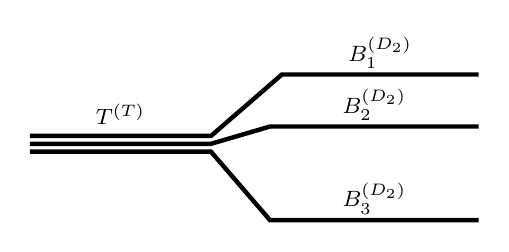
\begin{tikzpicture}
		\draw [ultra thick] (0,0.1) -- (2.3,0.1) node[above,midway] {\footnotesize $T^{(T)}$}-- (3.2,0.88) -- (5.7,0.88) node[above,midway,yshift=-2pt] {\footnotesize $B_1^{(D_2)}$};
		\draw [ultra thick] (0,0) -- (2.3,0) -- (3.05,0.22) -- (5.7,0.22) node[above,midway,yshift=-2pt] {\footnotesize $B_2^{(D_2)}$};
		\draw [ultra thick] (0,-0.1) -- (2.3,-0.1) -- (3.05,-0.97) -- (5.7,-0.97) node[above,midway,yshift=-2pt] {\footnotesize $B_3^{(D_2)}$};
	\end{tikzpicture}
\end{document}